\documentclass[a4paper, 12pt, final, garamond]{book}
\usepackage{cours-preambule}

\raggedbottom

\makeatletter
\renewcommand{\@chapapp}{M\'ecanique -- chapitre}
\makeatother

\begin{document}
\setcounter{chapter}{1}

\chapter{TD~: Dynamique du point}

% \section{Curling}
% Une pierre de curling est lancée sur une piste glacée horizontale selon un axe
% donné. Sa vitesse initiale vaut $v_0 = \SI{3.0}{m.s^{-1}}$. À cause des
% frottements, elle subit une \textit{décélération} constante $a_0 =
% \SI{0.1}{m.s^{2}}$ lors de son mouvement rectiligne. \bigbreak
% \begin{enumerate}
%     \item Au bout de combien de temps la pierre s'arrête-t-elle~?
%     \item Quelle distance a-t-elle parcouru~?
% \end{enumerate}

\section{Collision entre deux voitures}

Pendant le GP explorer organisé par Squeezie en octobre 2022, Pierre suit Xari
de près en vue de le dépasser. On considère ici que les deux voitures se suivent
sur une ligne droite à la vitesse de $v_0 = \SI{30}{m.s^{-1}}$ à une distance $d
= \SI{20}{m}$ l'une de l'autre. À la date $t=0$, la première freine avec une
décélération constante $a_1 = \SI{-20,0}{m.s^{-2}}$. Celle qui suit commence son
freinage $\tau = \SI{1}{s}$ plus tard (à cause du temps de réaction du
conducteur), avec une décélération de $a_2 = \SI{-10,0}{m.s^{-2}}$. \bigbreak

\begin{enumerate}
    \item En prenant pour origine du repère spatial la position de la seconde
        voiture à la date $t=0$, établir les équations horaires du mouvement des
        deux véhicules.
    \item Déterminer la position $x_c$ et la date $t_c$ du contact. Pierre
        avait-il le temps d'esquiver Xari~?
\end{enumerate}

\section{Masse attachée à 2 ressorts}
\begin{minipage}{0.75\linewidth}
    On considère un point M de masse $m$ attaché à deux ressorts identiques
    verticaux, de constante de raideur $k$ et de longueur à vide $\ell_0$. Les
    deux autres extrémités O et O' des ressorts sont fixes et espacées d'une
    distance $L$. On définit l'axe (O$z$) vertical ascendant. \bigbreak
    \begin{enumerate}
        \item Déterminer la position d'équilibre $z_{\eq}$ de M.
        \item Déterminer l'équation différentielle à laquelle satisfait $z(t)$.
            On écrira cette équation en fonction de $\w_0$ à définir et de
            $z_{\eq}$.
        \item On écarte M d'une hauteur $a$ par rapport à sa position
            d'équilibre, et on le lâche sans vitesse. Déterminer $z(t)$.
    \end{enumerate}
\end{minipage}
\hfill
\begin{minipage}{0.18\linewidth}
    \begin{center}
        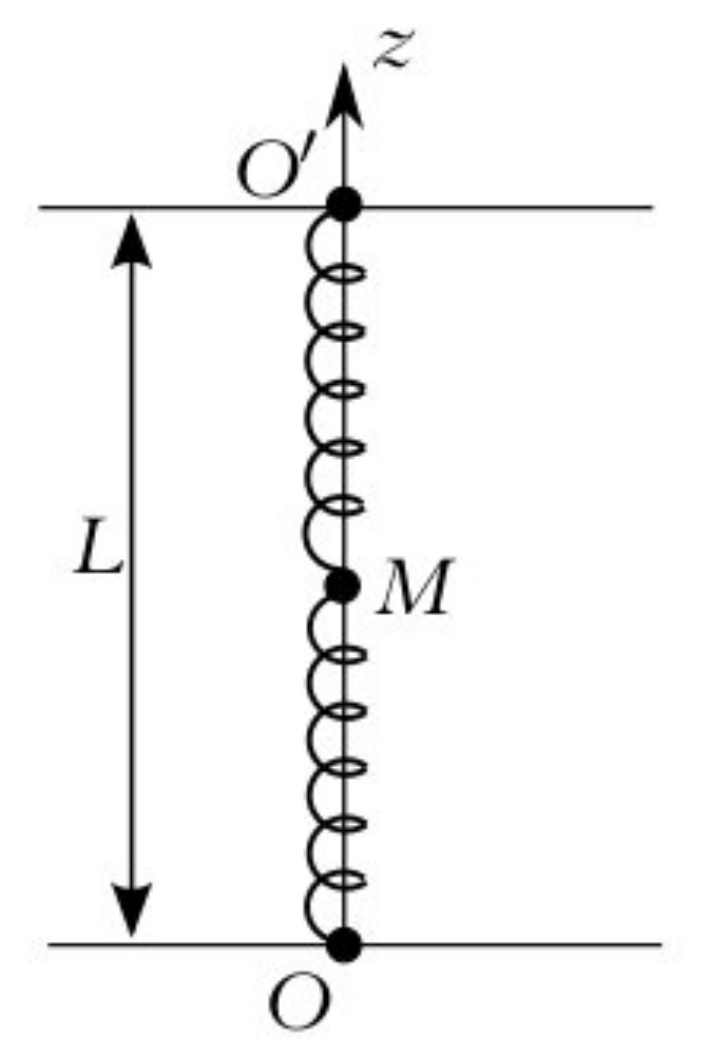
\includegraphics[width=\linewidth]{masse_2R-plain}  
    \end{center}
\end{minipage}

\section{Plan incliné et frottements solides}
\begin{minipage}{0.6\linewidth}
    On considère un plan incliné d'un angle $\alpha = \ang{20;;}$ par rapport à
    l'horizontale. Une brique de masse $m = \SI{600}{g}$ est lancée depuis le
    bas du plan vers le haut, avec une vitesse $v_0 = \SI{2.4}{m.s^{-1}}$. Pour
    étudier le mouvement, on utilise le repère (O,$x$,$y$) avec O coïncidant
    avec la position de départ de la brique. On note $g$ l'accélération de la
    pesanteur, avec $g = \SI{9.81}{m.s^{-2}}$. \bigbreak
\end{minipage}
\hfill
\begin{minipage}{0.35\linewidth}
    \begin{center}
        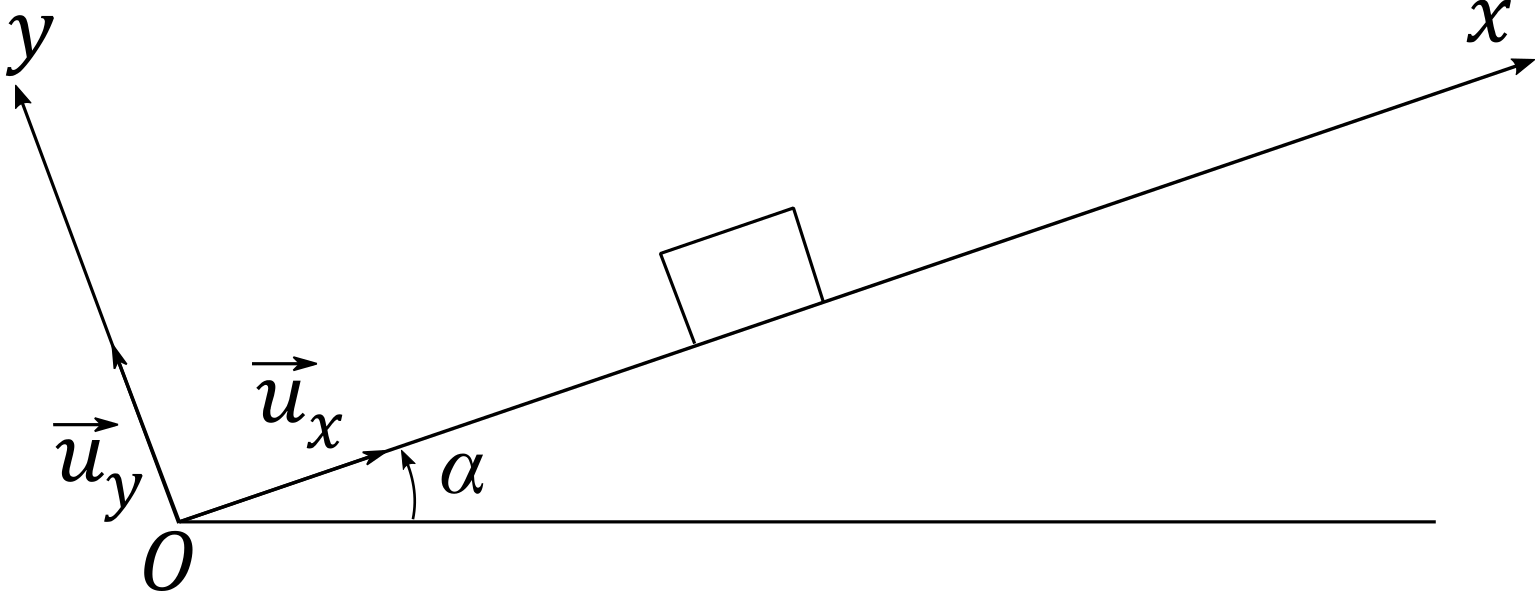
\includegraphics[width=\linewidth]{plan_incl-plain}
    \end{center}
\end{minipage}
\begin{enumerate}
    \item On suppose en premier lieu que le contact entre la brique et le plan
        incliné se fait sans frottements
        \begin{enumerate}
            \item Établir l'équation horaire du mouvement de la brique lors de
                sa montée.
            \item Déterminer la date à laquelle la brique s'arrête, ainsi que la
                distance qu'elle aura parcourue.
        \end{enumerate}
    \item On suppose ensuite qu'il existe des frottements solides, avec $f$ le
        coefficient de frottements solides tel que $f = \num{0.20}$.
        \begin{enumerate}
            \item Établir l'équation horaire du mouvement de la brique lors de
                sa montée.
            \item Déterminer la date à laquelle la brique s'arrête, ainsi que la
                distance qu'elle aura parcourue.
        \end{enumerate}
    \item On suppose finalement que la brique est \textbf{posée} sur le plan
        avec $\alpha$ variable.
        \begin{enumerate}
            \item Quel doit être l'angle $\alpha$ pour que l'objet se mette en
                mouvement~?
            \item Si le plan est en bois et la brique en métal, donner la valeur
                de cet angle. Même question si la brique est en bois. On donne
                \[
                    f_{\text{fer/chêne}} = \num{0.26}
                    \qet
                    f_{\text{chêne/chêne}} = \num{0.34}
                \]
        \end{enumerate}
    \item Avec $\alpha = \ang{0;;}$, on souhaite déplacer une armoire de
        \SI{100}{kg} en tirant dessus avec la force $\Ff$. On donne
        $f_{\text{armoire/sol}} = \num{0.25}$.
        \begin{enumerate}
            \item Déterminer la valeur de $\Ff$ pour mettre en mouvement
                l'armoire.
            \item En déduire à quoi sert de mettre des patins en téflon sur les
                pieds de l'armoire.
        \end{enumerate} 
\end{enumerate}

 % La réaction $\Rf$ du plan sur la brique s'exprime donc $\Rf = \Nf + \Tf$, avec
 % $\Tf$ colinéaire de sens contraire au vecteur vitesse

\section{Coup franc et frottements fluides}

\begin{minipage}{0.45\linewidth}
    On étudie dans le référentiel terrestre galiléen de repère fixe (O,$x$,$y$),
    un coup franc de football tiré à \SI{20}{m}, face au but de hauteur
    \SI{2,44}{m} et dans son plan médian vertical ($x$O$y$). L'axe (O$y$) est
    choisi suivant la verticale ascendante.
\end{minipage}
\hfill
\begin{minipage}{0.45\linewidth}
    \begin{center}
        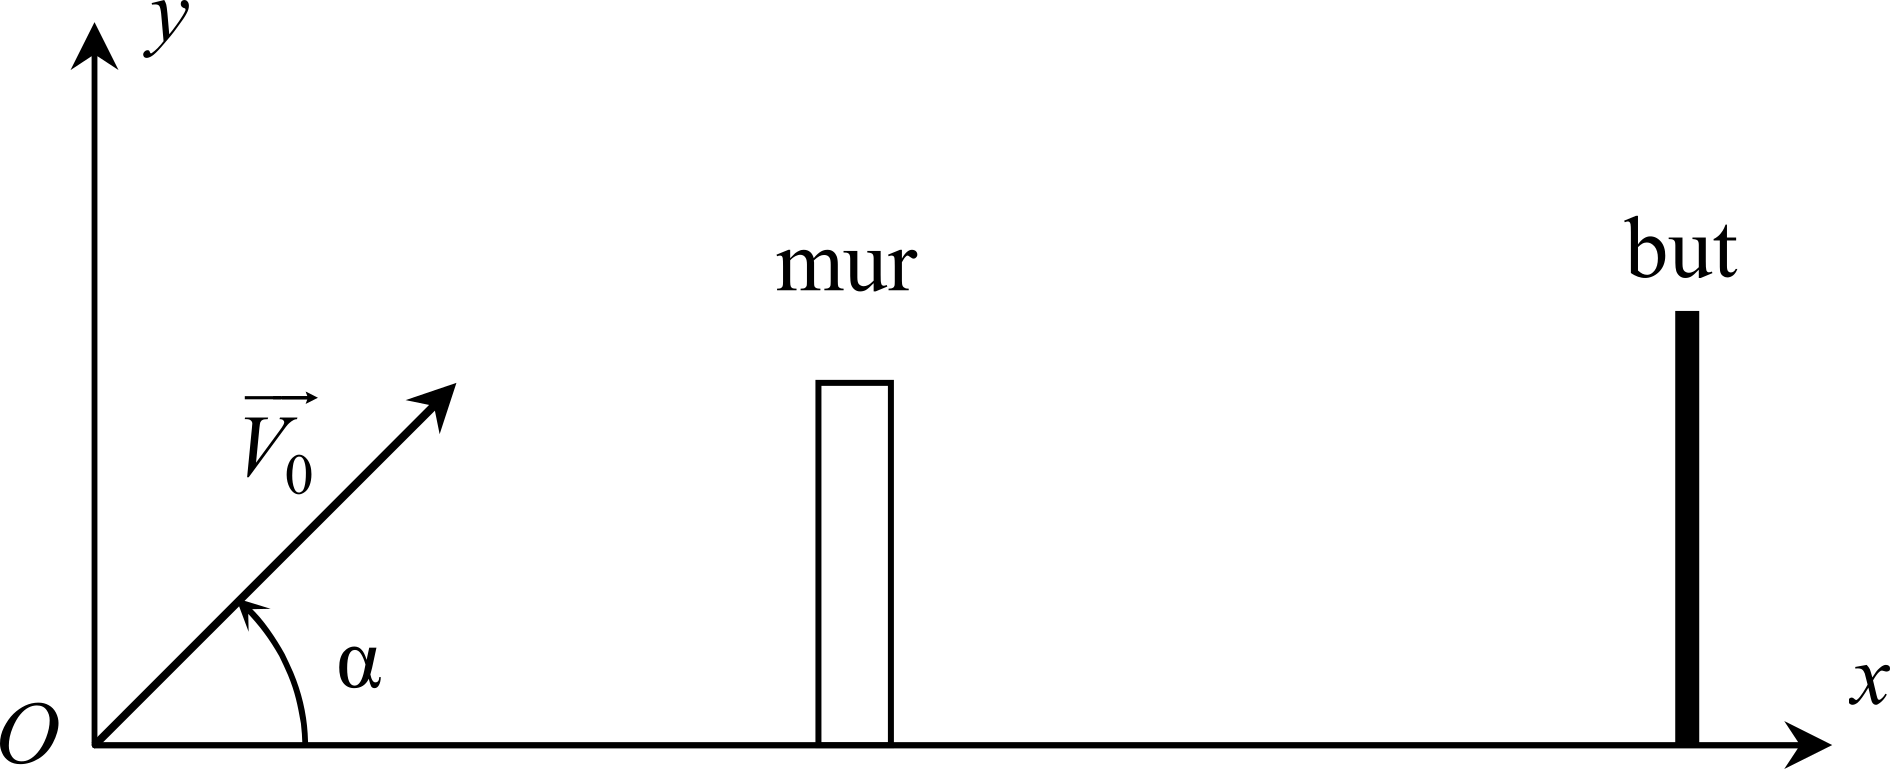
\includegraphics[width=\linewidth]{coup_franc-plain}
    \end{center}
\end{minipage}

Le ballon, de masse $m = \SI{430}{g}$, est assimilé à un point matériel M
initialement au sol en O. Le mur, de hauteur \SI{1,90}{m}, est situé à
\SI{9,15}{m} du ballon. Le ballon est lancé à l'instant $t = 0$ avec une vitesse
initiale $v_0$ de norme \SI{20}{m.s^{-1}} et formant un angle $\alpha$ de
\ang{20;;} avec l'horizontale. On note $g$ l'accélération de la pesanteur et on
rappelle que $g = \SI{9,81}{m.s^{-2}}$. \bigbreak
\begin{enumerate}
    \item Dans un premier temps, on néglige totalement les frottements de l'air.
        \begin{enumerate}
            \item Établir les équations horaires du mouvement du ballon ainsi
                que l'équation de la trajectoire.
            \item Le ballon passe-t-il au-dessus du mur~?
            \item Le tir est-il cadré~?
        \end{enumerate}
    \item Il y a en réalité des frottements, modélisés par une force $\Ff_f =
        -h\vf$ avec $h$ une constante positive de valeur
        \SI{5.00e-3}{kg.s^{-1}}.
        \begin{enumerate}
            \item Déterminer les équations horaires en introduisant la constante
                $\tau = \frac{m}{h}$.
            \item Donner l'équation de la trajectoire.
            \item Le ballon passe-t-il au-dessus du mur~?
            \item Le tir est-il cadré~?
        \end{enumerate}
\end{enumerate}

\section{Charge soulevée par une grue}

Une grue de chantier de hauteur $h$ doit déplacer d'un point à un autre du
chantier une charge M de masse $m$ supposée ponctuelle. On appelle A le point
d'attache du câble sur le chariot de la grue.

\begin{minipage}{0.45\linewidth}
    \begin{center}
        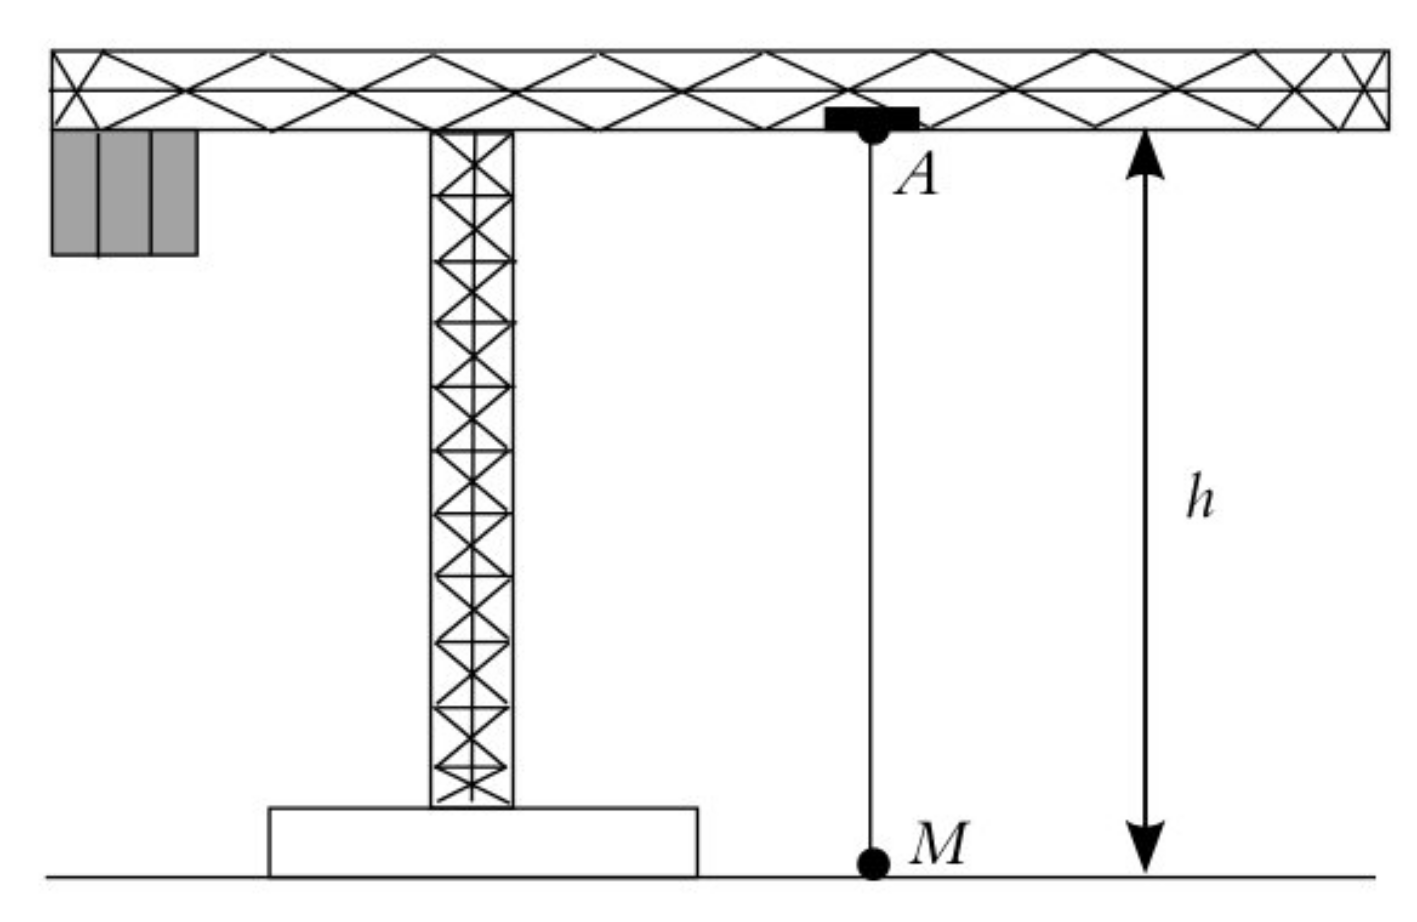
\includegraphics[height=3cm]{grue_fig1-plain}
        \captionof{figure}{Mouvement vertical}
    \end{center}
\end{minipage}
\hfill
\begin{minipage}{0.45\linewidth}
    \begin{center}
        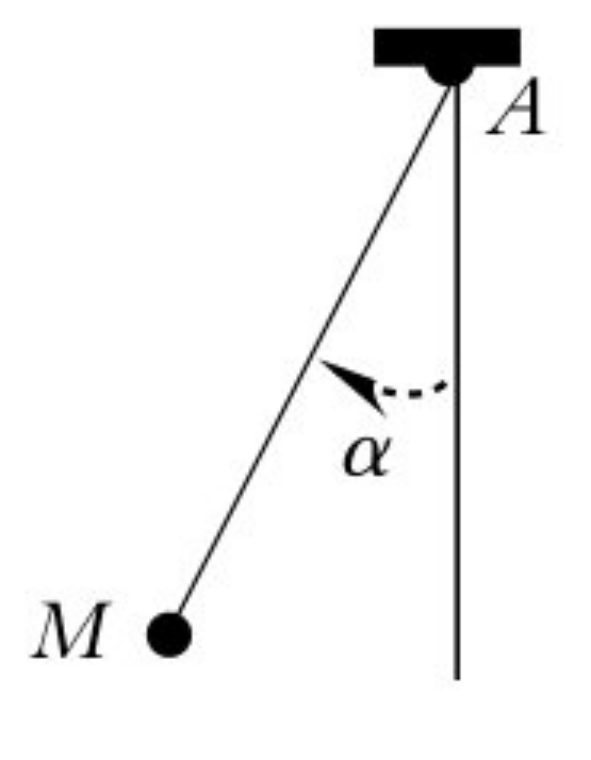
\includegraphics[height=3cm]{grue_fig2-plain}
        \captionof{figure}{Mouvement horizontal}
    \end{center}
\end{minipage}

\begin{enumerate}
    \item Le point A est à la verticale de M posée sur le sol. Déterminer la
        tension du câble lorsque M décolle (figure 1).
    \item L'enrouleur de câble de la grue remonte le câble avec une accélération
        $a_v$ constante. Déterminer la tension du câble et conclure.
    \item La montée de M est stoppée à mi-hauteur mais le chariot A se met en
        mouvement vers la droite (figure 2) avec une accélération $a_h$
        constante.
        \begin{enumerate}
            \item Quelle est l'accélération de M sachant que M est alors
                immobile par rapport à A~?
            \item Déterminer l'angle $\alpha$ (figure 2) que fait le câble avec
                la verticale en fonction de $m$, $g$, $a_h$ ainsi que la tension
                du câble.
        \end{enumerate}
\end{enumerate}

\section{Étude d'un volant de badminton}

Un volant de badminton a une masse $m = \SI{5,0}{g}$. On veut vérifier
expérimentalement l'information trouvée sur internet qui précise qu'un volant
lâché de très haut atteint une vitesse limite $v_l = \SI{25}{km.h^{−1}}$. Pour tester
cette affirmation, on veut déterminer l'altitude $h$ à laquelle il faut le lâcher
(sans vitesse initiale) pour qu'il atteigne cette vitesse limite. \bigbreak

On lâche le volant d'une fenêtre en hauteur et on filme sa chute verticale. On
note O le point de départ de la chute, et (O$z$) l'axe vertical dirigé vers le
bas. Au cours de la chute, on prend en compte une force de frottement due à
l'air de la forme $\Ff = -\lambda v\vf$ où $\vf$ est le vecteur vitesse du point
M, $v$ sa norme et $\lambda$ un coefficient positif. On note $g$ l'accélération
de la pesanteur et on rappelle que $g = \SI{9,81}{m.s^{−2}}$.

\begin{enumerate}
    \item Établir l'équation différentielle portant sur la norme du vecteur
        vitesse $v(t)$.
    \item Montrer l'existence d'une vitesse limite $v_l$ et l'exprimer en
        fonction de $\lambda$, $m$ et $g$.
\end{enumerate}
On note $t^* = t/\tau$, $z^* = z/L$ et $v^* = v/v_l$, avec $\tau = v_l/g$ et $L
= v_l\tau$.
\begin{enumerate}[resume]
    \item Montrer que $t^*$, $z^*$ et $v^*$ sont trois grandeurs sans dimension.
    \item Montrer que l'équation différentielle portant sur la vitesse peut se
        mettre sous la forme~:
        \[\dv{v^*}{t^*} + (v^*)^2 = 1\]
\end{enumerate}
La résolution de l'équation précédente conduit à des solutions dont on donne les
représentations graphiques ci-dessous.

\begin{center}
    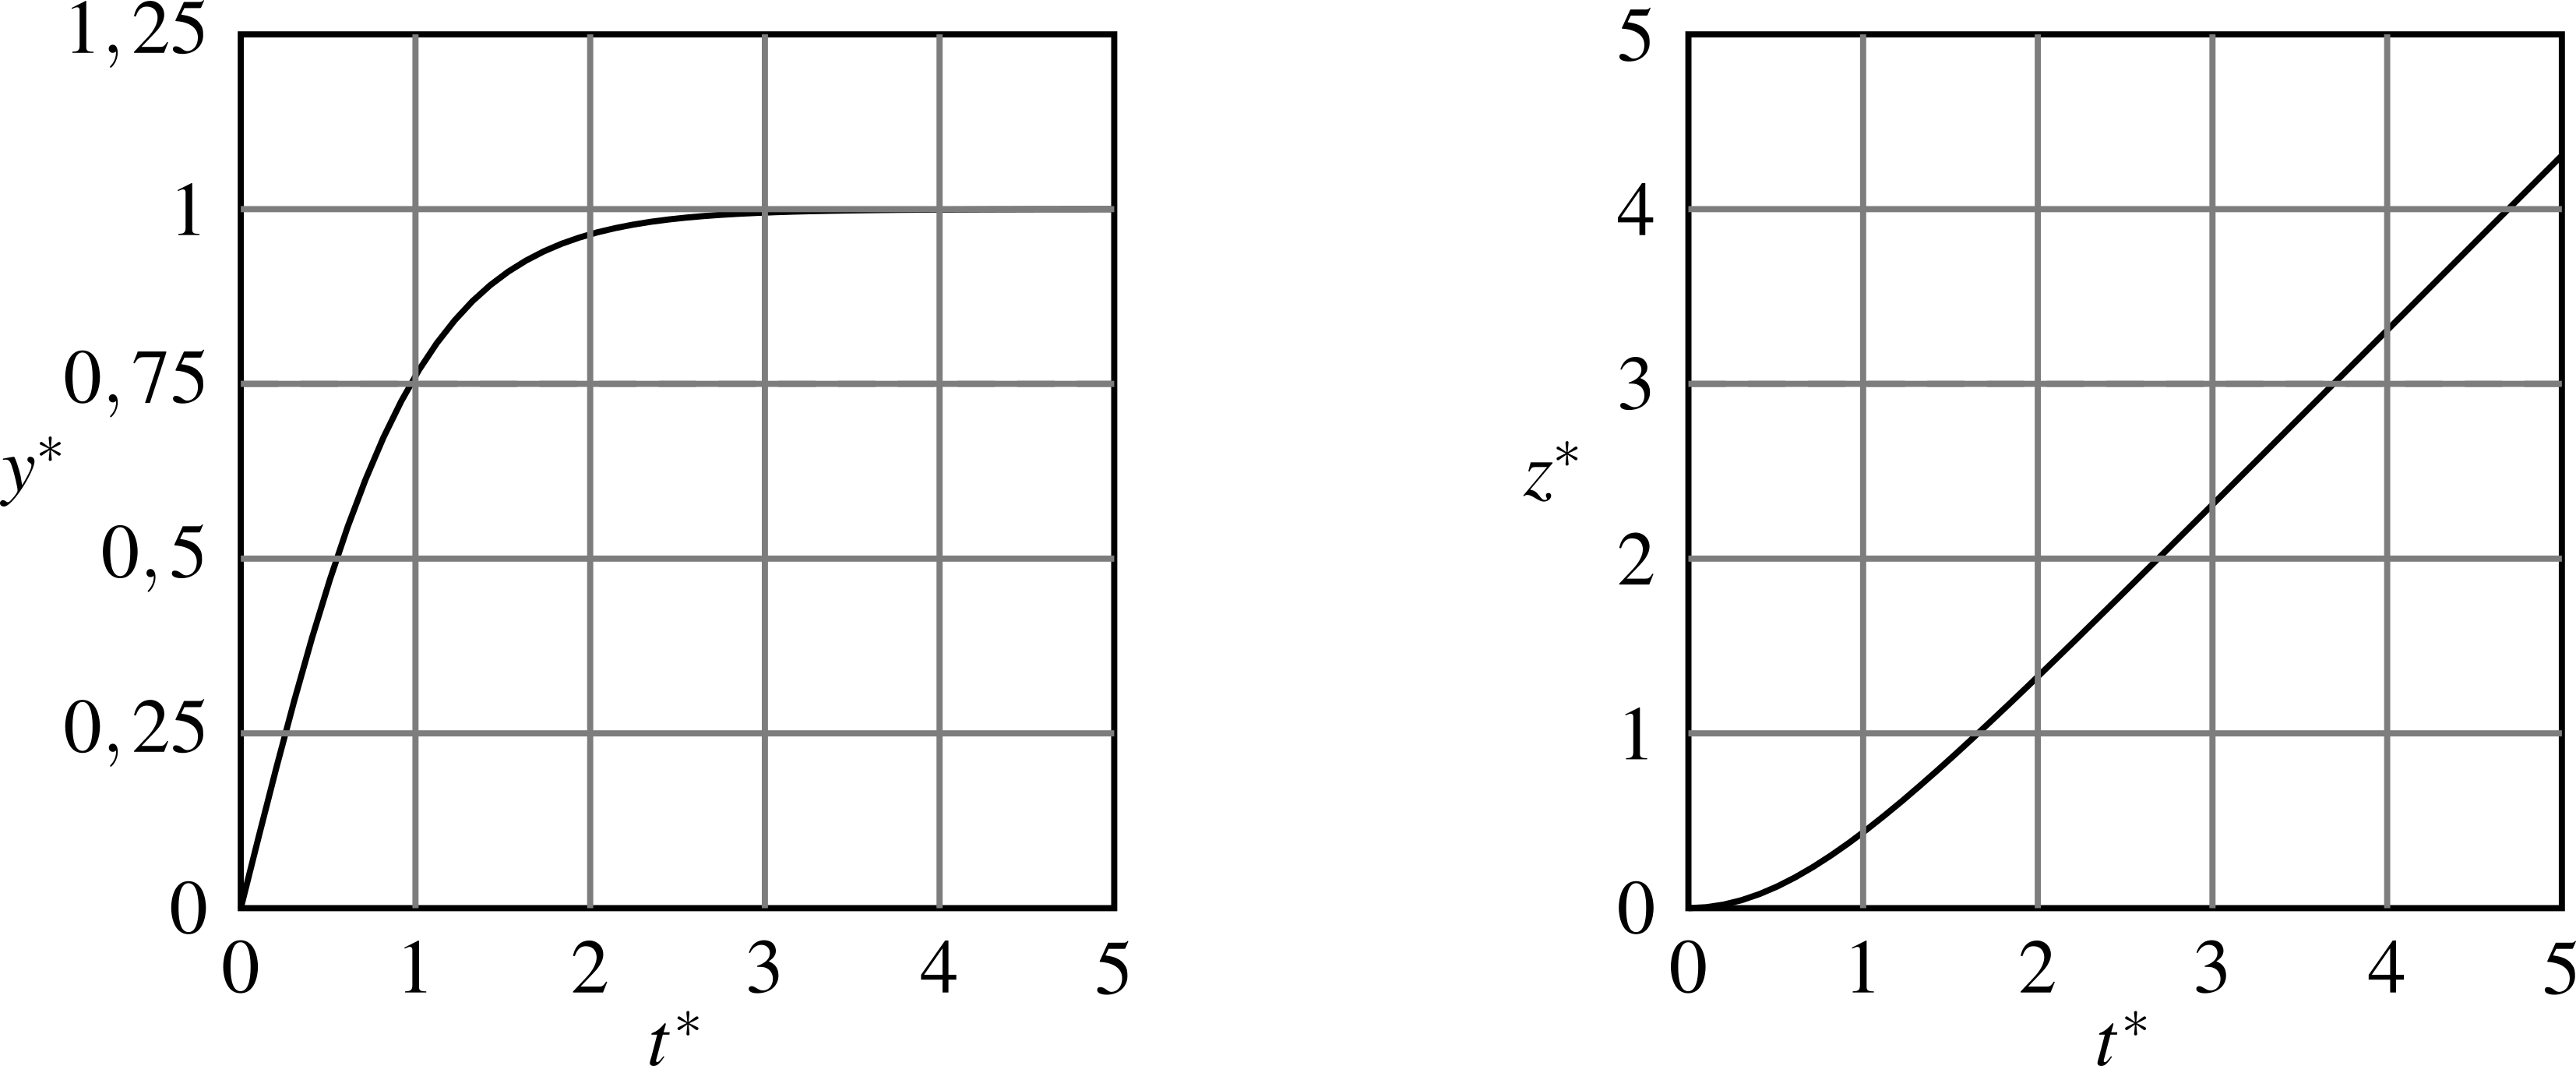
\includegraphics[width=.8\linewidth]{volant_data-plain}
\end{center}

\begin{enumerate}[resume]
    \item À l'aide des courbes, décrire les deux phases du mouvement.
    \item Déterminer l'altitude minimale $h$ à laquelle il faut lâcher le volant
        pour que sa vitesse au sol soit supérieure ou égale à 95\% de $v_l$. On
        exprimera cette altitude en fonction de $L$. Déterminer également la
        durée $\D t$ de l'expérience en fonction de $\tau$.
    \item En admettant que la vitesse limite est proche de la valeur trouvée sur
        internet, calculer numériquement $L$ et $\tau$ puis $h$ et $\Dt$.
\end{enumerate}

\section{Étude d'une skieuse}
On étudie le mouvement d'une skieuse descendant une piste selon la ligne de plus
grande pente, faisant un angle $\alpha$ avec l'horizontale. L'air exerce une
force de frottements supposée de la forme $\Ff = -\lambda\vf$ avec $\lambda$ un
coefficient positif et $\vf$ le vecteur vitesse du skieur. \bigbreak
On note $\Tf$ et $\Nf$ les composantes tangentielle et normale de la force de
frottements exercée par la neige, et $f$ le coefficient de frottements solides
tel que $\norm{\Tf} = f\norm{\Nf}$. \bigbreak
On choisit comme origine de l'axe (O$x$) de la ligne le plus grande pente la
position initiale de la skieuse, supposée partir à l'instant initiale avec une
vitesse négligeable. On note (O$y$) l'axe normal à la piste en O et dirigée vers
le haut.
\begin{enumerate}
    \item Calculer $\Tf$ et $\Nf$.
    \item Calculer la vitesse $\vf(t)$ et la position $x(t)$ de la skieuse à
        chaque instant $t$.
    \item Montrer que la skieuse atteint une vitesse limite $\vf_l$ et exprimer
        $\vf(t)$ et $\OM(t)$ en fonction de $\vf_l$.
    \item Calculer $v_l = \norm{\vf_l}$ pour $\lambda = \SI{1}{kg.s^{-1}}$, $f =
        \num{0.9}$, $g = \SI{10}{m.s^{-1}}$, $m = \SI{65}{kg}$ et $\alpha =
        \ang{45;;}$.
    \item Calculer littéralement et numériquement la date $t_1$ où la skieuse a
        une vitesse égale à $v_l/2$.
    \item À la date $t_1$, la skieuse chute. On néglige alors la résistance de
        l'air et on considère que le coefficient de frottements sur le sol est
        multiplié par 10. Calculer la distance parcourue par la skieuse avant
        qu'elle ne s'arrête.
\end{enumerate}

\end{document}
